\section{Inverse Trigonometric Functions}\label{sec:InvTrigFunctionsSection}
The trigonometric functions frequently arise in problems, and often it
is necessary to invert the functions, for example, to find an angle with
a specified sine. Of course, there are many angles with the same sine,
so the sine function doesn't actually have an inverse that reliably
``undoes'' the sine function. If you know that $\sin x=0.5$, you can't
reverse this to discover $x$, that is, you can't solve for
$x$, as there are infinitely many angles with sine
$0.5$. Nevertheless, it is useful to have something like an inverse to
the sine, however imperfect. The usual approach is to pick out some
collection of angles that produce all possible values of the sine
exactly once. If we ``discard'' all other angles, the resulting
function does have a proper inverse.

The sine takes on all values between $-1$ and $1$ exactly once on the
interval $[-\pi/2,\pi/2]$. 
$$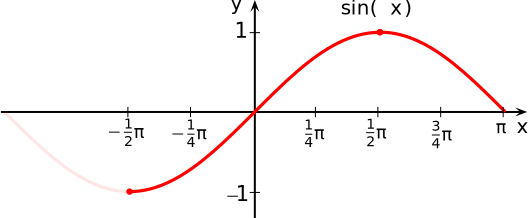
\includegraphics[width=4in]{images2/inv-trig-sin}$$
If we truncate the sine, keeping only the
interval $[-\pi/2,\pi/2]$, then this truncated sine has an inverse function. We call this
the inverse\index{inverse sine} sine or the arcsine\index{arcsine}, and
write it in one of two common notation: $y=\arcsin(x)$, or $y=\sin^{-1}(x)$.
$$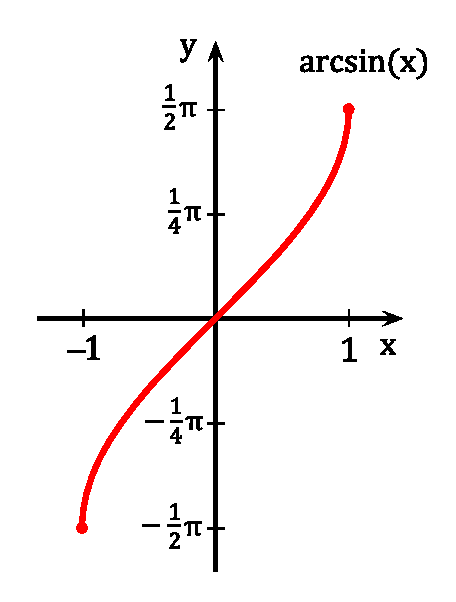
\includegraphics[width=2in]{images2/inv-trig-arcsin}$$

Recall that a function and its inverse undo each other in either
order, for example, $\ds (\root3\of x)^3=x$ and $\ds \root3\of{x^3}=x$. This
does not work with the sine and the ``inverse sine'' because the
inverse sine is the inverse of the truncated sine function, not the
real sine function. It is true that $\sin(\arcsin(x))=x$, that is, the
sine undoes the arcsine. It is not true that the arcsine undoes the
sine, for example, $\sin(5\pi/6)=1/2$ and $\arcsin(1/2)=\pi/6$, so
doing first the sine then the arcsine does not get us back where we
started. This is because $5\pi/6$ is not in the domain of the
truncated sine. If we start with an angle between $-\pi/2$ and $\pi/2$
then the arcsine does reverse the sine: $\sin(\pi/6)=1/2$ and
$\arcsin(1/2)=\pi/6$.

\begin{example}{Arcsine of Common Values}{Arcsine of Common Values}
Compute $\sin^{-1}(0)$,\quad $\sin^{-1}(1)$\quad and\quad $\sin^{-1}(-1)$.  
\end{example}

\begin{solution}
These come directly from the graph of $y=\arcsin x$:
$$\sin^{-1}\left( 0\right) =0\qquad \qquad \sin^{-1}(1)=\frac{\pi}{2}\qquad  \qquad \sin^{-1}(-1)=-\frac{\pi}{2}$$
\end{solution}

We can do something similar for the cosine function. As with the sine, we must
first truncate the cosine so that it can be inverted, in particular, we use the interval $[0,\pi]$. 
$$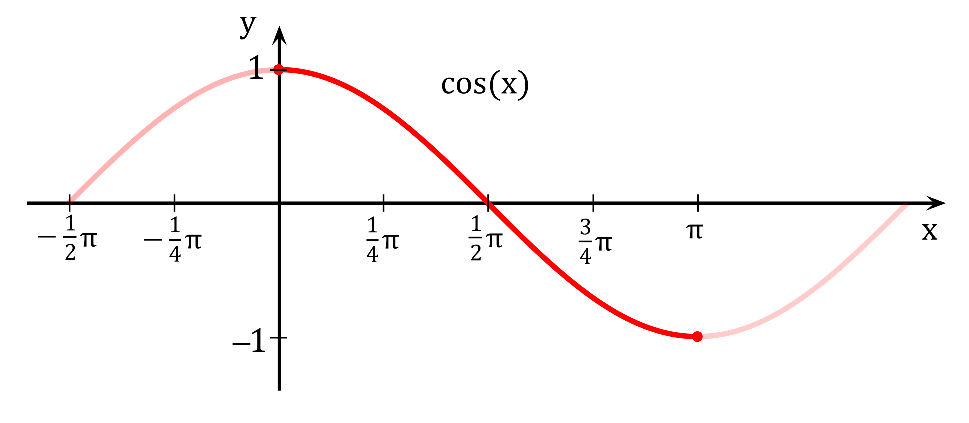
\includegraphics[width=4in]{images2/inv-trig-cos}$$
Note that the
truncated cosine uses a different interval than the truncated sine, so
that if $y=\arccos(x)$ we know that $0\le y\le \pi$.
$$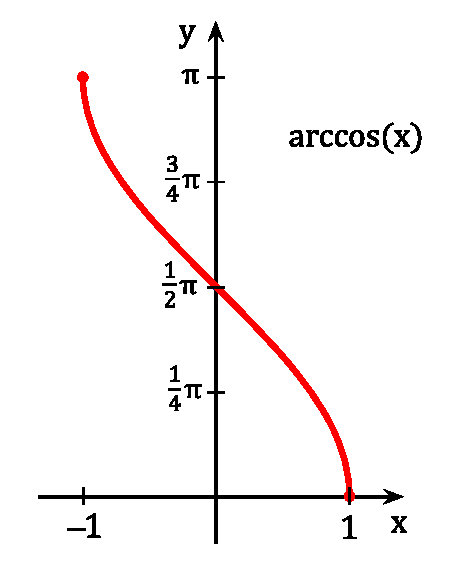
\includegraphics[width=2in]{images2/inv-trig-arccos}$$

\begin{example}{Arccosine of Common Values}{Arccosine of Common Values}
Compute $\cos^{-1}(0)$,\quad $\cos^{-1}(1)$\quad and\quad $\cos^{-1}(-1)$.  
\end{example}

\begin{solution}
These come directly from the graph of $y=\arccos x$:
$$\cos^{-1}\left( 0\right) =\frac{\pi}{2}\qquad \qquad \cos^{-1}(1)=0\qquad  \qquad \cos^{-1}(-1)=\pi$$
\end{solution}

Finally we look at the tangent; the other trigonometric functions also
have ``partial inverses'' but the sine, cosine and tangent are enough
for most purposes. The truncated tangent uses an interval of $(-\pi/2,\pi/2)$.
$$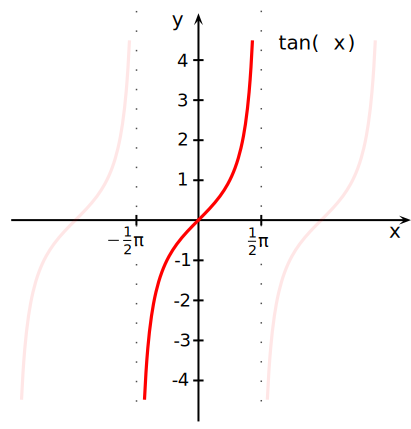
\includegraphics[width=2.75in]{images2/inv-trig-tan}$$
Reflecting the truncated tangent in the line $y=x$ gives the arctangent function.
$$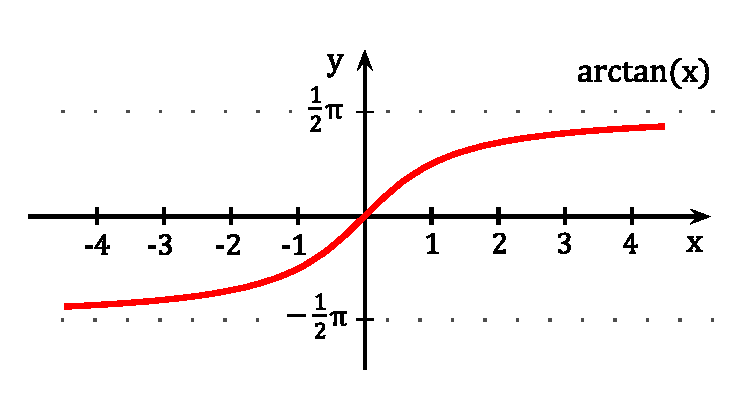
\includegraphics[width=3.5in]{images2/inv-trig-arctan}$$

\begin{example}{Arctangent of Common Values}{Arctangent of Common Values}
Compute $\tan^{-1}(0)$.
What value does $\tan^{-1}x$ approach as $x$ gets larger and larger?
What value does $\tan^{-1}x$ approach as $x$ gets large (and negative)? 
\end{example}

\begin{solution}
These come directly from the graph of $y=\arctan x$.
In particular, $\tan^{-1}(0)=0$.
As $x$ gets larger and larger, $\tan^{-1}x$ approaches a value of $\frac{\pi}{2}$, whereas, as $x$ gets large but negative, $\tan^{-1}x$ approaches a value of $-\frac{\pi}{2}$.
\end{solution}

The cancellation rules are tricky since we restricted the domains of the trigonometric functions in order to obtain inverse trig functions:

\begin{formulabox}[Cancellation Rules]
\[ \sin ( \sin^{-1} x ) = x, \ \ \ x \in [-1, 1] \qquad\qquad \sin^{-1} ( \sin x) = x, \ \ \ x \in \left[-\frac{\pi}{2}, \frac{\pi}{2} \right] \]
\[ \cos ( \cos^{-1} x ) = x, \ \ \ x \in [-1, 1] \qquad\qquad \ \ \ \cos^{-1} ( \cos x) = x, \ \ \ x \in \left[0, \pi \right]\ \ \  \]
\[ \tan ( \tan^{-1} x ) = x, \ \ \ x \in (-\infty, \infty) \qquad\qquad \tan^{-1} ( \tan x) = x, \ \ \ x \in \left(-\frac{\pi}{2}, \frac{\pi}{2} \right) \]
\end{formulabox}

\begin{example}{Arcsine of $1/2$}{Arcsine of $1/2$}
Find $\sin ^{-1}\left( 1/2\right) $. 
\end{example}

\begin{solution}
Since $\sin^{-1}(x)$ outputs values in $[-\pi/2,~\pi/2]$, the answer must be in this interval.
Let $\theta=\sin^{-1}(1/2)$. 
We need to compute $\theta$. 
Take the sine of both sides to get $\sin \theta = \sin(\sin^{-1}(1/2))=1/2$ by the cancellation rule.
There are many angles $\theta$ that work, but we want the one in the interval $[-\pi/2,~\pi/2]$.
Thus, $\theta=\pi/6$ and hence, $\ds\sin^{-1}\left(\frac{1}{2}\right)=\frac{\pi}{6}$.
\end{solution}

\begin{example}{Arccosine and the Cancellation Rule}{Arccosine and the Cancellation Rule}
Compute $\cos ^{-1}(\cos(0))$,\quad $\cos ^{-1}(\cos(\pi))$,\quad $\cos^{-1}(\cos(2\pi))$,\quad $\cos^{-1}(\cos(3\pi))$. 
\end{example}

\begin{solution}
Since $\cos^{-1}(x)$ outputs values in $[0,~\pi]$, the answers must be in this interval.  
The first two we can cancel using the cancellation rules:  
$$\cos ^{-1}(\cos(0))=0\qquad\mbox{and}\qquad\cos ^{-1}(\cos(\pi))=\pi.$$ 
The third one we cannot cancel since $2\pi\notin[0,\pi]$:
$$\cos ^{-1}(\cos(2\pi))\mbox{\quad\red{is NOT equal to}\quad}2\pi.$$  
But we know that cosine is a $2\pi$-periodic function, so $\cos(2\pi)=\cos(0)$: 
$$\cos ^{-1}(\cos(2\pi))=\cos^{-1}(\cos(0))=0$$
Similarly with the fourth one, we can \red{NOT} cancel yet since $3\pi\notin[0,\pi]$. Using $\cos(3\pi)=\cos(3\pi-2\pi)=\cos(\pi)$:  
$$\cos ^{-1}(\cos(3\pi))=\cos^{-1}(\cos(\pi))=\pi.$$
\end{solution}

\begin{example}{The Triangle Technique}{The Triangle Technique}
Rewrite the expression $\cos(\sin^{-1}x)$ without trig functions.
Note that the domain of this function is all $x\in[-1,1]$.
\end{example}

\begin{solution}
Let $\theta=\sin^{-1}x$. 
We need to compute $\cos\theta$.
Taking the sine of both sides gives $\sin \theta = \sin(\sin^{-1}(x))=x$ by the cancellation rule. 
We then draw a right triangle using $\sin\theta=x/1$:
$$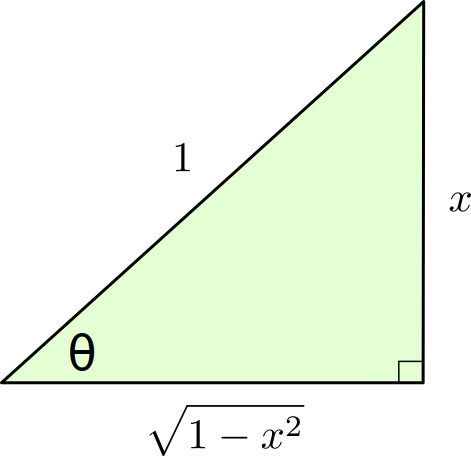
\includegraphics[width=1.5in]{images2/inv-trig-triangle-1}$$
If $z$ is the remaining side, then by the Pythagorean Theorem:
$$z^2+x^2=1\qquad\to\qquad z^2=1-x^2\qquad\to\qquad z=\pm\sqrt{1-x^2}$$
and hence $z=+\sqrt{1-x^2}$ since $\theta\in[-\pi/2,~\pi/2]$.
Thus, $\ds\cos\theta=\sqrt{1-x^2}$ by SOH CAH TOA, so, $\ds\cos(\sin^{-1}x)=\sqrt{1-x^2}$.
\end{solution}

\begin{example}{The Triangle Technique 2}{The Triangle Technique 2}
For $x\in(0,1)$, rewrite the expression $\ds\sin(2\cos^{-1}x)$.  
Compute $\sin(2\cos^{-1}(1/2))$. 
\end{example}

\begin{solution}
Let $\theta=\cos^{-1}x$ so that $\cos\theta = x$.  
The question now asks for us to compute $\sin(2\theta)$.  
We then draw a right triangle using $\cos\theta=x/1$:
$$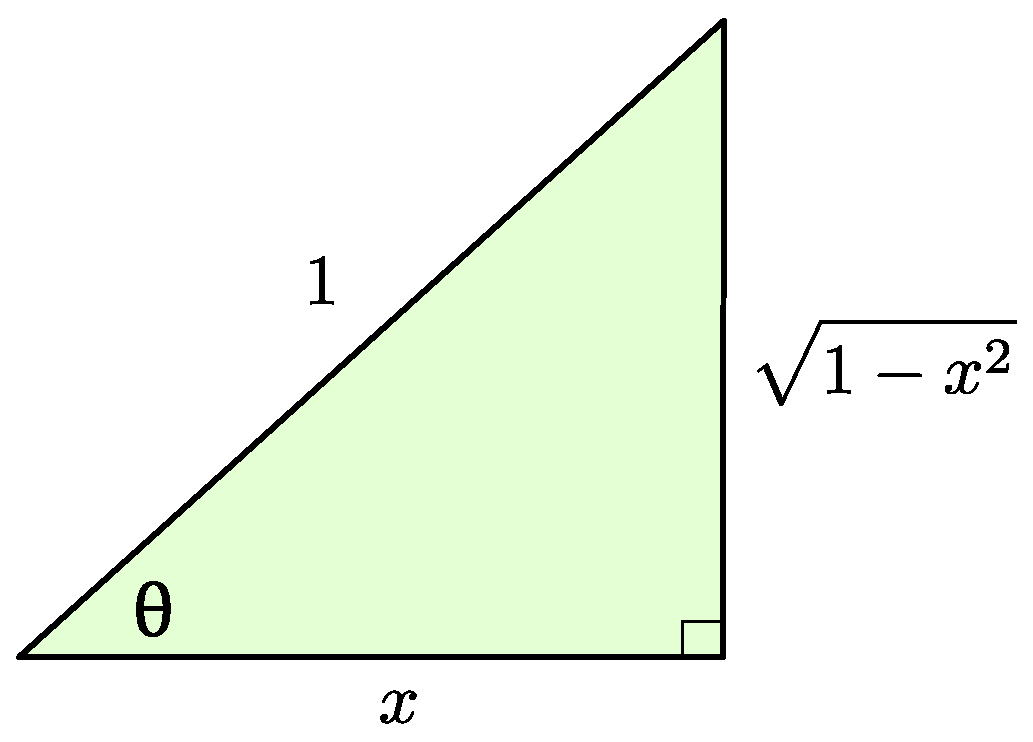
\includegraphics[width=1.75in]{images2/inv-trig-triangle-2}$$
To find $\sin(2\theta)$ we use the double angle formula $\ds \sin(2\theta)=2\sin\theta\cos\theta$.
But $\sin\theta=\sqrt{1-x^2}$, for $\theta\in[0,\pi]$, and $\cos\theta=x$. 
Therefore, $\ds\sin(2\cos^{-1}x)=2x\sqrt{1-x^2}$. 
When $x=1/2$ we have $\ds\sin(2\cos^{-1}(1/2))=\frac{\sqrt 3}{2}$.
\end{solution}


In Figure \ref{fig:domain_trig} we show the restrictions of the domains of the standard trigonometric functions that allow them to be invertible.\\

%\noindent %\hskip-110pt%
%\noindent\begin{minipage}{\textwidth+200pt}
\small\noindent
%\centering%\begin{center}
%\noindent\begin{minipage}[t]{.5\textwidth}%
\begin{tabular}{cccccc}
Function & Domain & Range &\parbox[b]{40pt}{\centering Inverse Function} & Domain & Range\\ \hline
\rule{0pt}{12pt} $\sin x$ & $[-\pi/2, \pi/2]$ & $[-1,1]$&$\sin^{-1} x$ & $[-1,1]$ & $[-\pi/2, \pi/2]$ \\
\rule{0pt}{12pt}$\cos x$ & $[0,\pi]$ & $[-1,1]$&$\cos^{-1}(x)$ & $[-1,1]$ & $[0,\pi]$ \\
\rule{0pt}{12pt}$\tan x$ & $(-\pi/2,\pi/2)$ & $(-\infty,\infty)$&$\tan^{-1}(x)$ & $(-\infty,\infty)$ & $(-\pi/2,\pi/2)$	\\
%\rule{0pt}{12pt} $\csc x$ & $[-\pi/2,0)\cup (0, \pi/2]$ & $(-\infty,-1]\cup [1,\infty)$&$\csc^{-1} x$ & $(-\infty,-1]\cup [1,\infty)$ & $[-\pi/2,0)\cup (0, \pi/2]$  \\
%the following makes integral of inverse function nicer
\rule{0pt}{12pt} $\csc x$ & $[-\pi/2,0)\cup (0, \pi/2]$ & $(-\infty,-1]\cup [1,\infty)$&$\csc^{-1} x$ & $(-\infty,-1]\cup [1,\infty)$ & $(0,\pi/2]\cup (\pi, 3\pi/2]$  \\
%\rule{0pt}{12pt}$\sec x$ & $[0,\pi/2)\cup (\pi/2,\pi]$ & $(-\infty,-1]\cup [1,\infty)$&$\sec^{-1}(x)$ & $(-\infty,-1]\cup [1,\infty)$ & $[0,\pi/2)\cup (\pi/2,\pi]$ \\
%the following makes integral of inverse function nicer
\rule{0pt}{12pt}$\sec x$ & $[0,\pi/2)\cup (\pi/2,\pi]$ & $(-\infty,-1]\cup [1,\infty)$&$\sec^{-1}(x)$ & $(-\infty,-1]\cup [1,\infty)$ & $[0,\pi/2)\cup [\pi,3\pi/2]$ \\
\rule{0pt}{12pt}$\cot x$ & $(0,\pi)$ & $(-\infty,\infty)$&$\cot^{-1}(x)$ &  $ (-\infty,\infty)$ & $(0,\pi)$	
\end{tabular}
%\captionsetup{type=figure}
\caption{Domains and ranges of the trigonometric and inverse trigonometric functions.}\label{fig:domain_trig}
%\end{center}
%\normalsize
%\end{minipage}
%\captionsetup{type=figure}%
%\caption{Domains and ranges of the trigonometric and inverse trigonometric functions.}\label{fig:domain_trig}
%\end{minipage}
%}
%%%%%%%%%%%%%%%%%%%%%%%%%%%%%%%%%%%%%%%%%%%%
\Opensolutionfile{solutions}[ex]
\section*{Exercises for \ref{sec:InvTrigFunctionsSection}}

\begin{enumialphparenastyle}

\begin{ex}
Compute the following:
\begin{multicols}{2}
\begin{enumerate}
	\item	$\sin^{-1}(\sqrt{3}/2)$
	\item	$\cos^{-1}(-\sqrt{2}/2)$
\end{enumerate}
\end{multicols}
\begin{sol}
\begin{enumerate}
	\item	$\pi/3$
	\item	$3\pi/4$
\end{enumerate}
\end{sol}
\end{ex}

\begin{ex}
Compute the following:
\begin{multicols}{2}
\begin{enumerate}
	\item	$\sin^{-1}\left(\sin(\pi/4)\right)$
	\item	$\sin^{-1}\left(\sin(17\pi/3)\right)$
	\item	$\cos\left(\cos^{-1}(1/3)\right)$
	\item	$\tan\left(\cos^{-1}(-4/5)\right)$
\end{enumerate}
\end{multicols}
\begin{sol}
\begin{multicols}{2}
\begin{enumerate}
	\item	$\pi/4$
	\item	$-\pi/3$
	\item	$1/3$
	\item	$-3/4$
\end{enumerate}
\end{multicols}
\end{sol}
\end{ex}

\begin{ex}
Rewrite the expression $\tan\left(\cos^{-1}x\right)$
without trigonometric functions. What is the domain of this function?
\begin{sol}
$\sqrt{1-x^2}/x$ with domain $[-1,0)\cup(0,1]$.
\end{sol}
\end{ex}

\end{enumialphparenastyle}